\chapwithtoc{Introduction}
\label{chap:intro}

Ray tracing is a powerful image synthesis technique used in 3D computer graphics, capable of simulating optical effects, such as reflection, refraction, and scattering, with a high degree of visual realism. For this reason, it offers a variety of applications in the entertainment industry, it is used for product design, visual prototyping, and for creating visualizations in scientific research \cite [91-128]{peddie2019ray}. Reasons for the popularity of ray tracing algorithms are the physical plausibility of its generated images as well as their simplicity and "elegance". 

The origins of ray tracing can be traced back as far as 1968. At that time, a method was invented to shade wire-framed solids by shooting random light rays from virtual light sources to the scene geometry and, if an intersection would be found, placing a symbol at the intersection point \cite{appel1968some}. If enough rays were generated, there would be a high concentration of these symbols at regions with high light intensity, which would approximate physical realism. A decade later, an elaboration of this idea to a shading model that takes global information into account for calculating light intensities  \cite{whitted1979improved}, would revolutionize the computer graphics field.

\begin{figure} \label{fig:whitted_result}
	\centering
	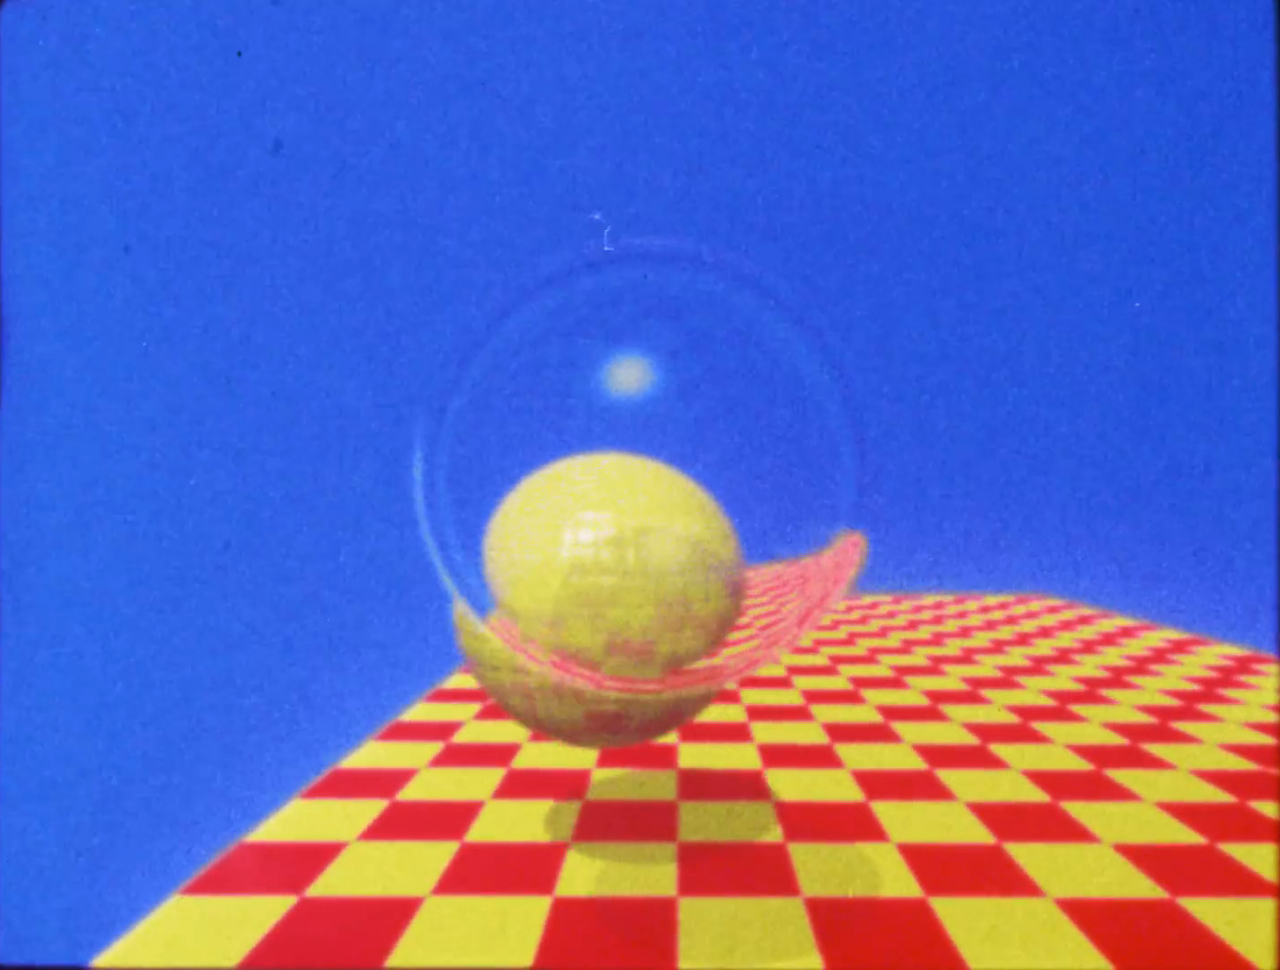
\includegraphics[width=.7\linewidth]{img/0 introduction/whitted_}
	\caption{A frame of the animation used to demonstrate the recursive ray tracer described in \cite{whitted1979improved}\cite{raytracingvideo}.}
	\label{fig:g}
\end{figure}

The calculation of intersection points between cast rays and scene geometry is a crucial part of ray tracing. How these points are calculated depends on the representation of geometric primitives in the scene. Primitives can be represented analytically or approximated by polygon meshes. Another possibility is the representation of a shape as a \emph{Constructive Solid Geometry (CSG)}. CSG is a hierarchical ordering of a set of primitive shapes to which Boolean set operations have been applied to. This form of representation enjoys popularity in e.g. Computer-aided geometric design.

Over the years, novel ray tracing algorithms that were inspired by this model came to be, aiming to increase physical correctness in rendered images. However, ray tracing remains to this day a computationally demanding task. Much research was (and still is) devoted to accelerating the ray tracing procedure to compensate for its computational expense. A variety of ray acceleration data structures and faster intersection algorithms were introduced. Furthermore, ray tracing is by nature is "embarrassingly parallel", meaning it is well suited for parallel processing by automatic vectorization. As Moore’s law predicted, the computational power in CPUs gradually increased. Nowadays, modern computers admit an integrated circuit with multiple cores on which the workload of the ray tracing algorithm can be distributed. While ray tracing was considered impractical when it was pioneered, it has now become accessible to everyone with a moderate laptop or PC, thanks to this development.

Despite this, exploiting the computational power of modern processors to their full potential for ray tracing remains challenging. This particular reason served as the motivation for developing the award-winning (\cite{embreeAward}), open-source framework \emph{Embree} \cite{wald2014embree}. Embree offers a set of ray tracing kernels that maximize the compute capabilities of modern x86 CPU architectures. The kernels are accessible to programmers by a provided API. 

One of the design goals behind Embree was an easy integration of the framework into existing professional ray tracing environments to achieve high performance when ray tracing virtual scenes with high geometrical complexity.


\section*{Thesis subject and motivation}
The goal of this thesis is a successful integration of the Embree framework into the rendering engine \emph{The Advanced Rendering Toolkit} \cite{artSoftware} (which will be referred to with its abbreviation \emph{ART} throughout this thesis), to facilitate the acceleration of the ray casting procedure for constructive solid geometry performed by ART.

ART offers innovative features, such as spectral rendering support, proper handling of bi-spectral materials (e.g., fluorescent surfaces) \cite{mojzik2018handling} and a physically plausible sky dome lighting model \cite{wilkie2013predicting}. Until the release of Mitsuba 2 \cite{nimier2019mitsuba}, ART was, to our best knowledge, the sole rendering system that would support rendering polarization effects. These features make ART an interesting environment for computer graphics researchers interested in the field of \emph{Predictive Rendering}.

ART provides a documented scene description language to facilitate these features, support for the rendering of various geometry primitive types, and functionality for importing PLY meshes as geometry objects. Furthermore, in this scene description language, one has to specify a so-called \emph{Action Sequence}, which can be thought of as a pipeline, directing how ART processes a given scene.
All this allows for great flexibility. However, to ensure this functionality, ART relies on its very own scene description data structures that diverge from those present in other popular rendering systems (e.g., pbrt \cite{pharr2016physically} or Mitsuba 2).


Although Embree was developed with the intention of it being "used in existing renderers with minimal programmer effort" \cite[1]{wald2014embree}, its integration into the CSG rendering framework ART is a non-trivial task on account of its internal data structures and since there is no direct support for CSG geometry by Embree.

The successful integration of Embree into ART would elevate a complex image synthesis system with unique features regarding spectral rendering to modern ray tracing standards. 

\section*{Thesis outline}

This thesis is structured as follows: 

\textbf{Chapter \ref{chap:fundamentals}} will provide fundamental background information including a brief introduction to the ray tracing technique, explanations of the most common ray acceleration structures, and a brief overview of functionality of the Embree framework.

In \textbf{Chapter \ref{chap:art}} provides a brief introduction to ART, in which Embree will be integrated into. This introduction focuses on the aspects of ART that are important for the comprehension of our integration approach.

\textbf{Chapter \ref{chap:integration}} is dedicated to the description of our approach on the integration of Embree into ART, as well as the implementation of the CSG operations with Embree.

The integration approach is then evaluated and obtained results are discussed in \textbf{Chapter \ref{chap:results}}  

The work of this thesis is concluded in \textbf{Chapter \ref{chap:conclusion}}.

Finally, \textbf{Appendix \ref{sec:embree_app}} provides a user guide for compiling ART with Embree support.